% This is samplepaper.tex, a sample chapter demonstrating the
% LLNCS macro package for Springer Computer Science proceedings;
% Version 2.20 of 2017/10/04
%
\documentclass{report}
%\documentclass[runningheads]{llncs}
%
\usepackage{graphicx}
\usepackage{algorithm}
\usepackage[spanish]{babel}
\usepackage[noend]{algpseudocode}
\usepackage{amsmath}
% Used for displaying a sample figure. If possible, figure files should
% be included in EPS format.
%
% If you use the hyperref package, please uncomment the following line
% to display URLs in blue roman font according to Springer's eBook style:
% \renewcommand\UrlFont{\color{blue}\rmfamily}

\begin{document}
%

\begin{titlepage}
\centering
{\bfseries\LARGE Instituto Nacional de Astrofísica Óptica y Electrónica \par}
\vspace{1cm}
{\scshape\Large Maestría en Ciencias Computacionales \par}
\vspace{3cm}
{\scshape\Huge Análisis Estadístico  \par}
\vspace{3cm}
{\itshape\Large Proyecto Estadística \par}
\vfill
{\Large Autor: \par}
{\Large Eliú Moreno Ramírez\par}
\vfill
{\Large Noviembre 2022 \par}
\end{titlepage}
           % typeset the header of the contribution
%

%
%
%
\textbf{Resumen}\\
El presente trabajo presenta un análisis estadístico para reforzar la teoría vista en clase y aprender cómo aplicarla para que en futuros proyectos sea más natural el uso de herramientas como python, el cual es un lenguaje hecho para el data science, esta práctica se calcularán medidas descriptivas, frecuencias y tablas de frecuencias todo esto se realizará con un estudio de muestras de hilo (Technometrics 1982:63)
\section{Introducción}
El análisis de datos estadísticos es el proceso que nos permite interpretar los datos numéricos que disponemos, con el objetivo de tomar las decisiones más eficaces. De hecho,las empresas pueden tomar decisiones 5 veces más rápido que su competencia si las basan en el análisis de datos~\cite{ref_article0}.\\
Existen muchas herramientas para el análisis de datos estadísticos, Excel el cual es principal para oficinistas, sin embargo existen lenguajes de programación especializados para la estadística, aquellos usados por excelencia son \textit{R} el es un entorno de software libre (licencia GNU GLP) y lenguaje de programación interpretado, es decir, ejecuta las instrucciones directamente, sin una previa compilación del programa a instrucciones en lenguaje máquina~\cite{ref_article1}; y \textit{Python} la analítica de Python se refiere a aplicaciones de analítica avanzada que utilizan Python, un lenguaje de programación de código abierto. Python es uno de los lenguajes de codificación líderes en la actualidad para la analítica de datos con una amplia gama de casos de uso empresarial en diversas industrias~\cite{ref_article2}.
Así que con este software el cual es libre, muchos investigadores así como analistas en la industria hacen uso para sus datos. Tomando estos antecedentes se hará un estudio estadístico para un pequeño problema del estudio de ruptura de la urdimbre durante el tejido de telas (Technometrics, 1982:63).
\section{Problemática}
El problema a estudiar es el siguiente: En un estudio de ruptura de la urdimbre durante el tejido de telas(Technometrics, 1982:63), se sometieron a prueba 100 muestras de hilo. Se determinó el número de ciclos de esfuerzo hasta ruptura para cada muestra de hilo y se obtuvieron unos datos.\\
Para este análisis se hará una tabla donde estas 100 muestras se clasificarán en clases, donde cada clase es un intervalo de longitud 85. También se harán gráficas de frecuencias(las cuales se detallan en la sección de soluciones propuestas).
\section{Objetivo}
La motivación de este trabajo es además de reforzar la parte teórica de estadística vista en clase, sino también para poder aplicar los aprendido ya que en el mundo actual para un análisis de este tipo generalmente ya se usa una cantidad de datos que son intratables para el ser humano por lo que se vuelve una necesidad aprender el uso de estas herramientas. Con el fin de ir aprendiendo el uso de este software se realizará un pequeño análisis de la problemática previa.
\section{Solución Propuesta}
Como ya mencionamos \textit{python} es una buena herramienta de trabajo en el uso estadístico, así que para el trabajo se harán uso de librerías como \textit{pandas}, \textit{matplotlib}, \textit{numpy} y \textit{seaborn}; con la versión de 3.9. Con el uso de estas librerías se realizará una tabla que contendrá intervalos de longitud 85, donde podremos encontrar ciertas medidas descriptivas tales como: esperanza matemática, media, mediana, moda, varianza, desviación estándar, primer momento, segundo momento, tercer momento; como segunda parte será crear una tabla que contenga distribución de frecuencias absoluta, frecuencia acumulada, frecuencia relativa, frecuencia relativa acumulada, frecuencia relativa, frecuencia relativa acumulada y la frecuencia porcentaje; además de que se puedan calcular los percentiles de estos datos; como tercera y última parte consistirá de gráficas las cuales nos permiten analizar estos datos de manera más visual, aquellas que se realizarán son gráfica de barras, histograma de frecuencia, polígono de frecuencia, diagrama de caja y gráfica de bastón.
\section{Desarrollo}
Para el cálculo de las medidas descriptivas se hizo mediante lo siguiente:
\begin{equation}
\begin{split}
Esperanza &= \sum_{-\infty}^{\infty} x \cdot f(x) dx\\
Momento_n &=E[(\frac{x-c}{b})^n]\\
Media &= \frac{\sum_{i=0}^{n}x_i}{n}
\end{split}
\end{equation}
Recordemos que la media, la esperanza matemática, primer momento es lo mismo; además de que la varianza es igual el segundo momento. La moda se calcula tomando aquel valor dentro de los datos que tiene mayor frecuencia. La desviación estándar es igual a la raíz cuadrada de la varianza.


\begin{equation}
\begin{split}
Rango & = X_{max}-X_{min} \\
Intervalos_i & = (X_{min}\times i,X_{min}\times (i+1))\\
MarcaClase_i &=(Intervalos_i[limire superior]-Intervalos_i[limire inferior])/2\\
Percentil_k &= Lp_k+\frac{n(\frac{k}{100})-F_{i-1}}{f_i}\times A
\end{split}
\end{equation}
Una vez calculado lo anterior podemos crear nuestra tabla de frecuencias así como nuestras gráficas, estas pueden verse en la figura[1].

\begin{figure}
\label{fig1}
\caption{Graficas del conjunto de datos del problema a analizar}
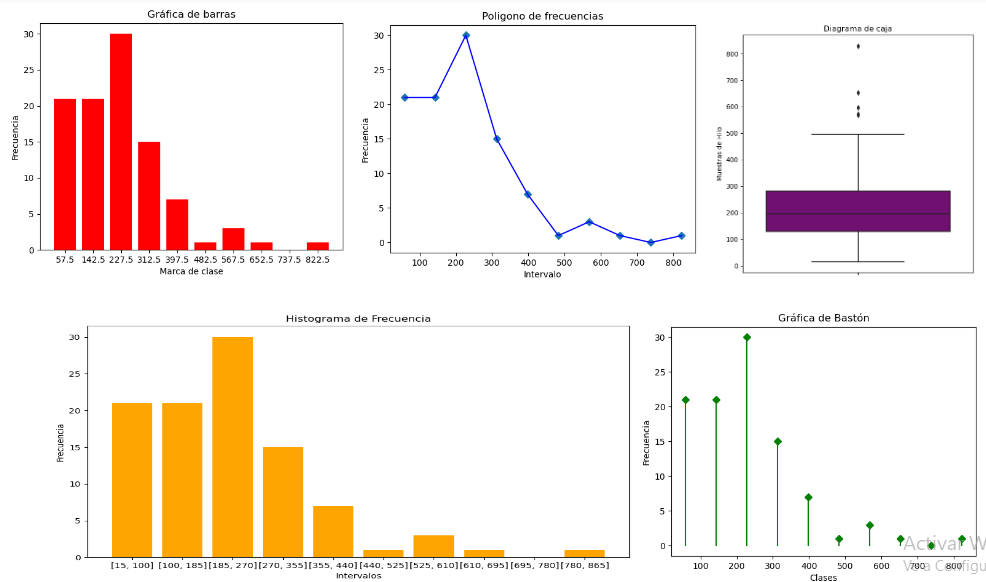
\includegraphics[width=1.1\textwidth]{images/1.png}
\end{figure}
\section{Conclusiones}
Como podemos ver en este documento el uso de este software es muy útil y eficiente para estos análisis, así que como se mencionó en el objetivo es importante aprender a aplicar la estadística ya que es una manera en la cual podemos estar preparados en la industria o la investigación, además actualmente es importante no sólo dominar la teoría sino dominar el cómo hacer uso de ésto. 

\begin{thebibliography}{8}

\bibitem{ref_article0} 
Piratoba Gil, R. P. Alarcón Guarín, Mg. R. (2011, octubre). Importancia de la estadística en una investigación cualitativa.
\bibitem{ref_article1}
Unir, V. (2020, 28 septiembre). Lenguaje R, ¿qué es y por qué es tan usado en Big Data? UNIR. https://www.unir.net/ingenieria/revista/lenguaje-r-big-data/
\bibitem{ref_article2}
¿Qué es la analítica Python? (s. f.). TIBCO Software. https://www.tibco.com/es/reference-center/what-are-python-analytics
\end{thebibliography}
\end{document}
